
\documentclass[a4paper,11pt]{article}
\usepackage[polish]{babel}
\usepackage[OT4]{fontenc}
\usepackage[utf8]{inputenc}
\usepackage{graphicx}
\usepackage{subfig}
\usepackage{epstopdf}




\date{06/05/2014}


%opening
\title{PAMSI -- testowanie algorytmów wyszukiwania w grafie}
\author{Piotr Wilkosz}
\captionsetup{belowskip=12pt,aboveskip=4pt}
\begin{document}

\maketitle

\section{Wstęp}
Celem ćwiczenia było przetestowanie implementacji algorytmów wyszukiwania ścieżki w grafie. Graf został stworzony 
na podstawie listy incydencji. Przetestowano następujące algorytmy:
  \begin{itemize}
   \item Przeszukiwanie wgłąb - DFS
   \item Przeszukiwanie wszerz - BFS
   \item Przeszukiwanie grafu poczynając od najkrótszej ścieżki - Best - First Search
   \item Algorytm A*
  \end{itemize}
Zadaniem było zmierzenie czasu wykonywania operacji wyszukania losowego elementu w grafie.
\section{Wyniki pomiarów}
\begin{enumerate}
 \item DFS
   
  \begin{table}[th]
  \centering
    \caption{Pomiar czasu przeszukiwania wgłąb w grafie}

      \begin{tabular}{|l|l|l|}
	\hline
	N & czas & odchylenie \\
    \hline
 10 & 0.00110325 & 0.000130398\\
 \hline
100 & 0.0274422 & 0.00285908\\
\hline
1000 & 0.134149 & 0.0233129\\
\hline
10000 & 3.41307 & 1.98324\\
\hline
50000 & 36.1375 & 11.0835\\
\hline
100000 & 54.0686 & 16.6036\\
\hline
    \end{tabular}
    \label{tab1}
    \end{table}
    \newpage
 \begin{figure}[th]
\centering
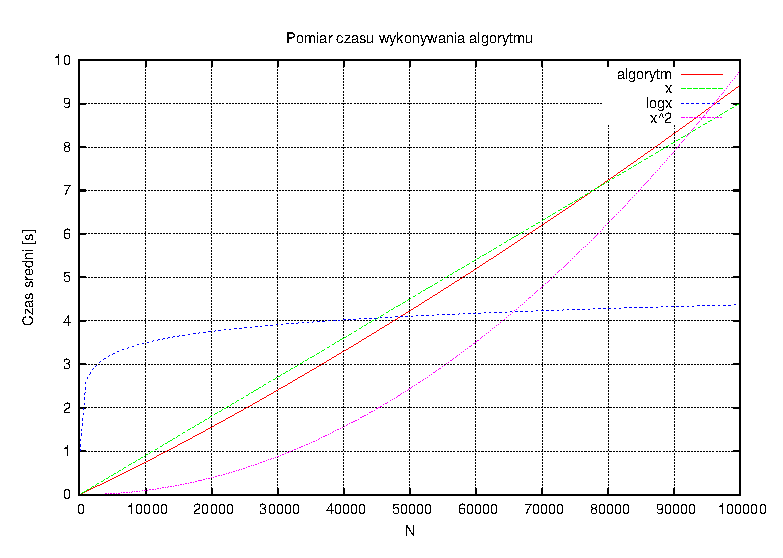
\includegraphics[width=0.8\textwidth]{../prj/wykres13.eps}
\caption{Wykres do tabeli nr 1}
\label{Wykres1}
\end{figure} 
Na podstawie wykresu\ref{Wykres1} i tabeli~\ref{tab1} czas operacji przeszukiwania wgłąb szacuje się jako liniowy. Duże odchylenie od średniego czasu przeszukiwania świadczy o tym,
 iż zarówno przypadek pesymistyczny, jak i optymistyczny przypada z jendakowym prawdopodbieństwem, co powoduje znaczące zróżnicowanie.
\item BFS
  \begin{table}[th]
  \centering
  
    \caption{Pomiar czasu przeszukiwania wszerz w grafie}

      \begin{tabular}{|l|l|l|}
	\hline
	N & czas & odchylenie \\
    \hline
10 & 0.000492332 & 4.54287e-05\\
\hline
100 & 0.00385789 & 0.000494668\\
\hline
1000 & 0.116186 & 0.0625103\\
\hline
10000 & 4.10229 & 1.92677\\
\hline
50000 & 27.1518 & 10.3526\\
\hline
100000 & 54.1763 & 20.0539\\
\hline
    \end{tabular}
    \label{tab2}
    \end{table}
    \newpage
\begin{figure}[th]
\centering
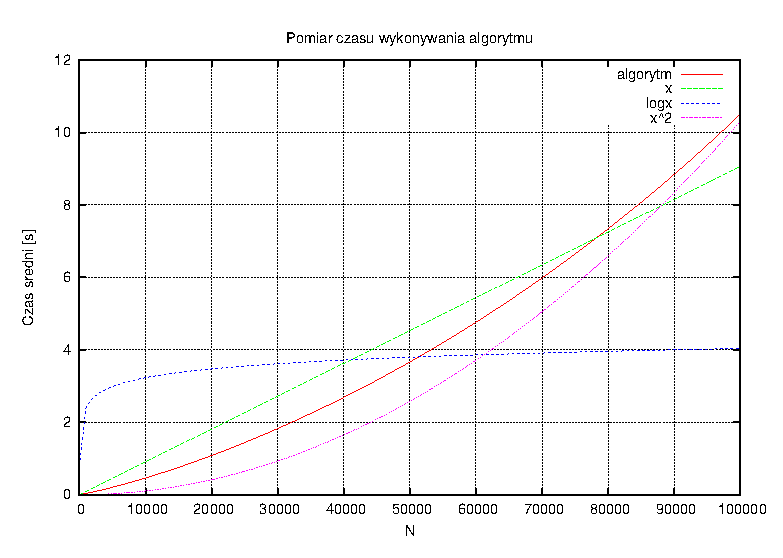
\includegraphics[width=0.8\textwidth]{../prj/wykres14.eps}
\caption{Wykres do tabeli nr 2}
\label{Wykres2}
\end{figure} 
Na podstawie wykresu~\ref{Wykres2} i tabeli~\ref{tab2} czas operacji przeszukiwania wszerz szacuje się jako liniowy. Podobnie jak w przypadku wcześniejszym, zaobserwować można 
spore odchylenie, jednak uśrednienie wyników daje czas proporcjonalny do sumy liczb wierzchołków i krawędzi w grafie.
\item Best - First Search

\begin{table}[th]
\centering
    \caption{Pomiar czasu przeszukiwania typu best - first w grafie}

      \begin{tabular}{|l|l|l|}
	\hline
	N & czas & odchylenie \\
    \hline
10 & 0.000659847 & 6.09969e-05\\
\hline
100 & 0.0108403 & 0.000987436\\
\hline
1000 & 0.358854 & 0.217304\\
\hline
10000 & 5.71089 & 2.71159\\
\hline
50000 & 25.7899 & 13.9438\\
\hline
100000 & 58.4636 & 24.0813\\
\hline
    \end{tabular}
    \label{tab3}
    \end{table}
    \newpage

    \begin{figure}[th]
\centering
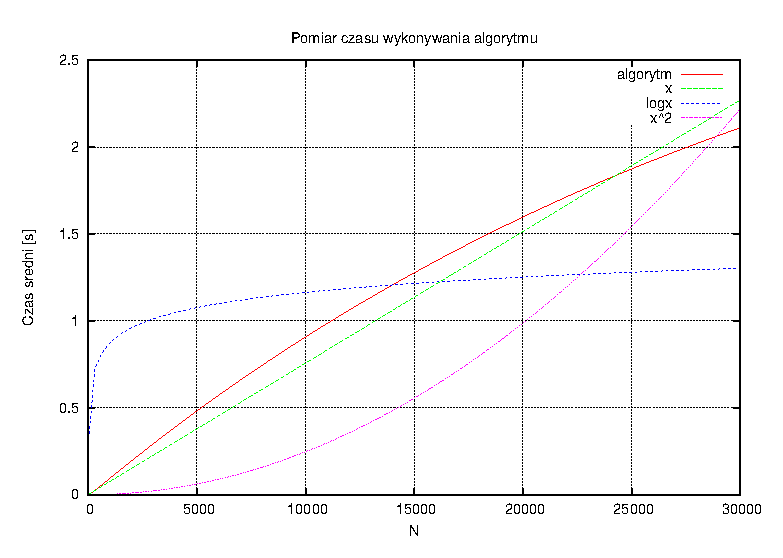
\includegraphics[width=0.8\textwidth]{../prj/wykres15.eps}
\caption{Wykres do tabeli nr 3}
\label{Wykres3}
\end{figure} 
Z danych z wykresu~\ref{Wykres3} i tabeli\ref{tab3} wyciągnąć podobne wnioski jak w przypadku dwóch poprzednich algorytmów. Czas wykonania operacji jest liniowy.

\item Algorytm A*

Algorytm A* służy do znajdowania najkrótszej ścieżki w grafie. W przeciwieństwie do powyższych algorytmów, nie podaje dowolnej ścieżki, lecz 
możliwie najkrótszą. Oczywiście dokładność tego algorytmu zależy od przyjętej heurystyki, im szacowana odległość jest bliższa rzeczywistej, tym lepszą 
ściezkę wskaże algorytm. Na potrzeby ćwiczenia zaimplementowano reprezentację grafu, która wspomagana była przez rozmieszczenie wierzchołków 
na płaszczyźnie kartezjańskiej. Do wyznaczania heurystyki użyto tzw. metryki typu Manhattan. W metryce tej odległość wyznacza się poprzez 
sumę odległości przebytych w linii prostej i poziomej. Ponadto długości ścieżek wybierane są losowo, gdzie najkrótsza możliwa odległość jest równa  
szacowanej odległości pomiędzy dwoma punktami, co zapobiega przeszacowaniu heurystyki.

\begin{table}[th]
\centering
    \caption{Pomiar czasu działania algorytmu A* w grafie}

      \begin{tabular}{|l|l|l|}
	\hline
	N & czas & odchylenie \\
    \hline
10 & 0.00104789 & 0.000782535\\
\hline
100 & 0.021713 & 0.00951804\\
\hline
1000 & 0.177888 & 0.13306\\
\hline
10000 & 15.6215 & 31.3469\\
\hline
50000 & 80.7123 & 88.6142\\
\hline
    \end{tabular}
    \label{tab4}
    \end{table}
    \newpage

    \begin{figure}[th]
\centering
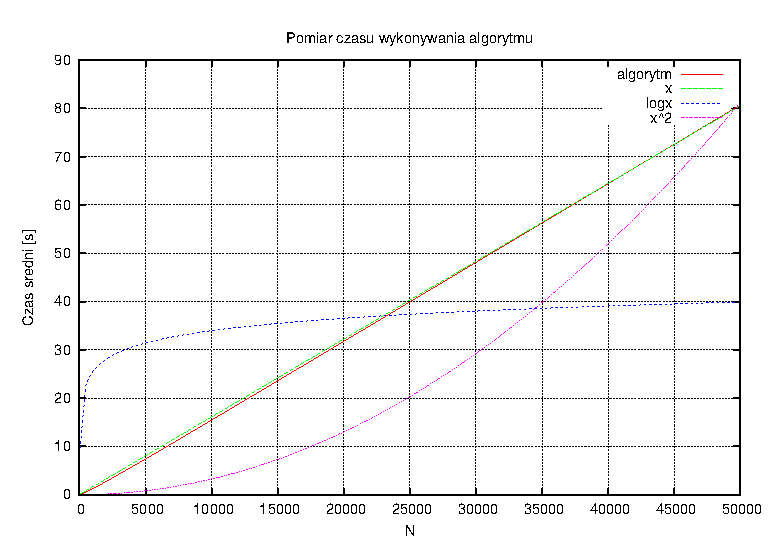
\includegraphics[width=0.8\textwidth]{../prj/wykres16.eps}
\caption{Wykres do tabeli nr 4}
\label{Wykres4}
\end{figure} 
Z danych z wykresu~\ref{Wykres4} i tabeli~\ref{tab4} mozna wyciągnąć podobne wnioski jak w przypadku dwóch poprzednich algorytmów. Czas wykonania operacji jest wprost proporcjonalny do sumy ilości węzłów oraz krawędzi.

\subsection{Zależność szybkości algorytmu A* od dokładności heurystyki}

Działanie algorytmu A* w istotny sposób zależy od jakości oszacowania drogi potrzebnej do przebycia pomiędzy danymi punktami. Poniżej umieszczono 
wykres przedstawiający szybkość działania algorytmu A* w zależności od stopnia dokładności heurystyki. 
Jak już wcześniej wspomniano, długość ścieżki pomiędzy dwoma punktami jest przydzielana losowo, lecz programista ma możliwość ustalenia 
maksymalnej różnicy pomiędzy oszacowaniem a rzeczywistą długością. Tak więc za miarę dokładności heurystyki można przyjąć maksymalną różnicę długości 
drogi oszacowanej i drogi rzeczywistej. Pomiarów dokonano na próbie 10 000 węzłów grafu ze względu na długi czas wykonania algorytmu.

  \begin{figure}[th]
\centering
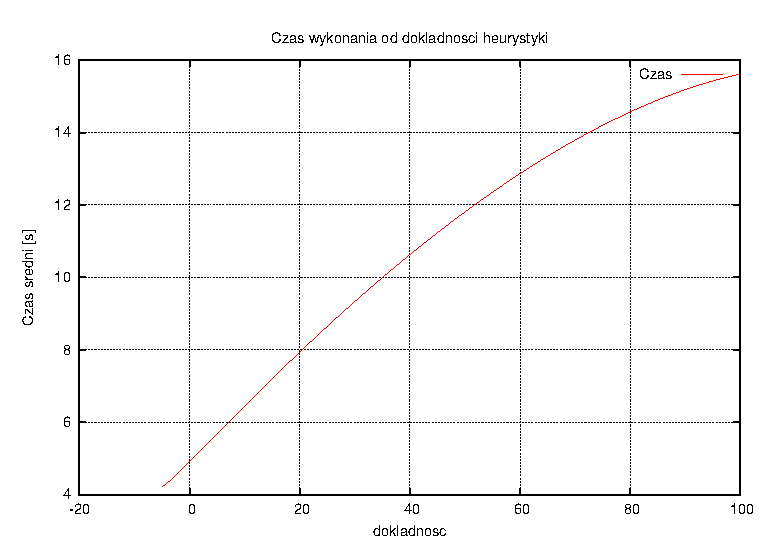
\includegraphics[width=0.8\textwidth]{../prj/wykres_a.eps}
\caption{Szybkość wykonania algorytmu A*}
\label{Wykres5}

Liczby na osi poziomej wykresu~\ref{Wykres5} to różnica pomiędzy rzeczywistą drogą a jej oszacowaniem zgodnie z zastosowaną metryką. Jak widać, im mniejsza jest ta różnica,
tym szybciej pracuje algorytm, gdy długość ścieżki estymujemy z nadmiarem, czas jest również krótszy, jednak możemy nie znaleźć najkrótszej ścieżki.
Powyższy wykres jest spójny z teorią, tzn. gdy heurystyka jest o wiele mniejsze od rzeczywistej długości, działanie algorytmu coraz bardziej zbliza się do algorytmu Dijkstry, w 
drugą stronę algorytm upodabnia się do tzw. best - first search.

\end{figure} 

\end{enumerate}

\section{Wnioski}

\begin{itemize}
\item Wszystkie powyższe algorytmy osiągają podobną złożoność obliczeniową.

\item wykorzystanie uprzednio stworzonych struktur danych, jak np. tablica asocjacyjna, pozwoliło na bardziej intuicyjną implementację algorytmów.

\item Niestety badane algorytmy mogą okazać się mało efektywnym sposobem przeszukiwania grafów. Efekty ich działania są zbyt mocno zależne od struktury grafu. O efektywności 
wykonania algorytmu w wielu sytuacjach decyduje losowe wybranie szukanego elementu, co często może prowadzić do sytuacji optymistycznej, ale także pesymistycznej.
\item Algorytm A* okazał się bardzo wydajnym algorytmem wyszukiwania najkrótszej ścieżki w grafie. Gdy potrafimy wyznaczyć dokładną heurystykę, algorytm łączy szybkość oraz 
możliwość optymalizacji (znalezienia najkrótszej ścieżki). Przyjęte oszacowanie ma wpływ na szybkość działania oraz na dokładność (dla przeszacowania algorytm może znalźć inną ścieżkę).

\end{itemize}

\begin{figure}[th]
\centering
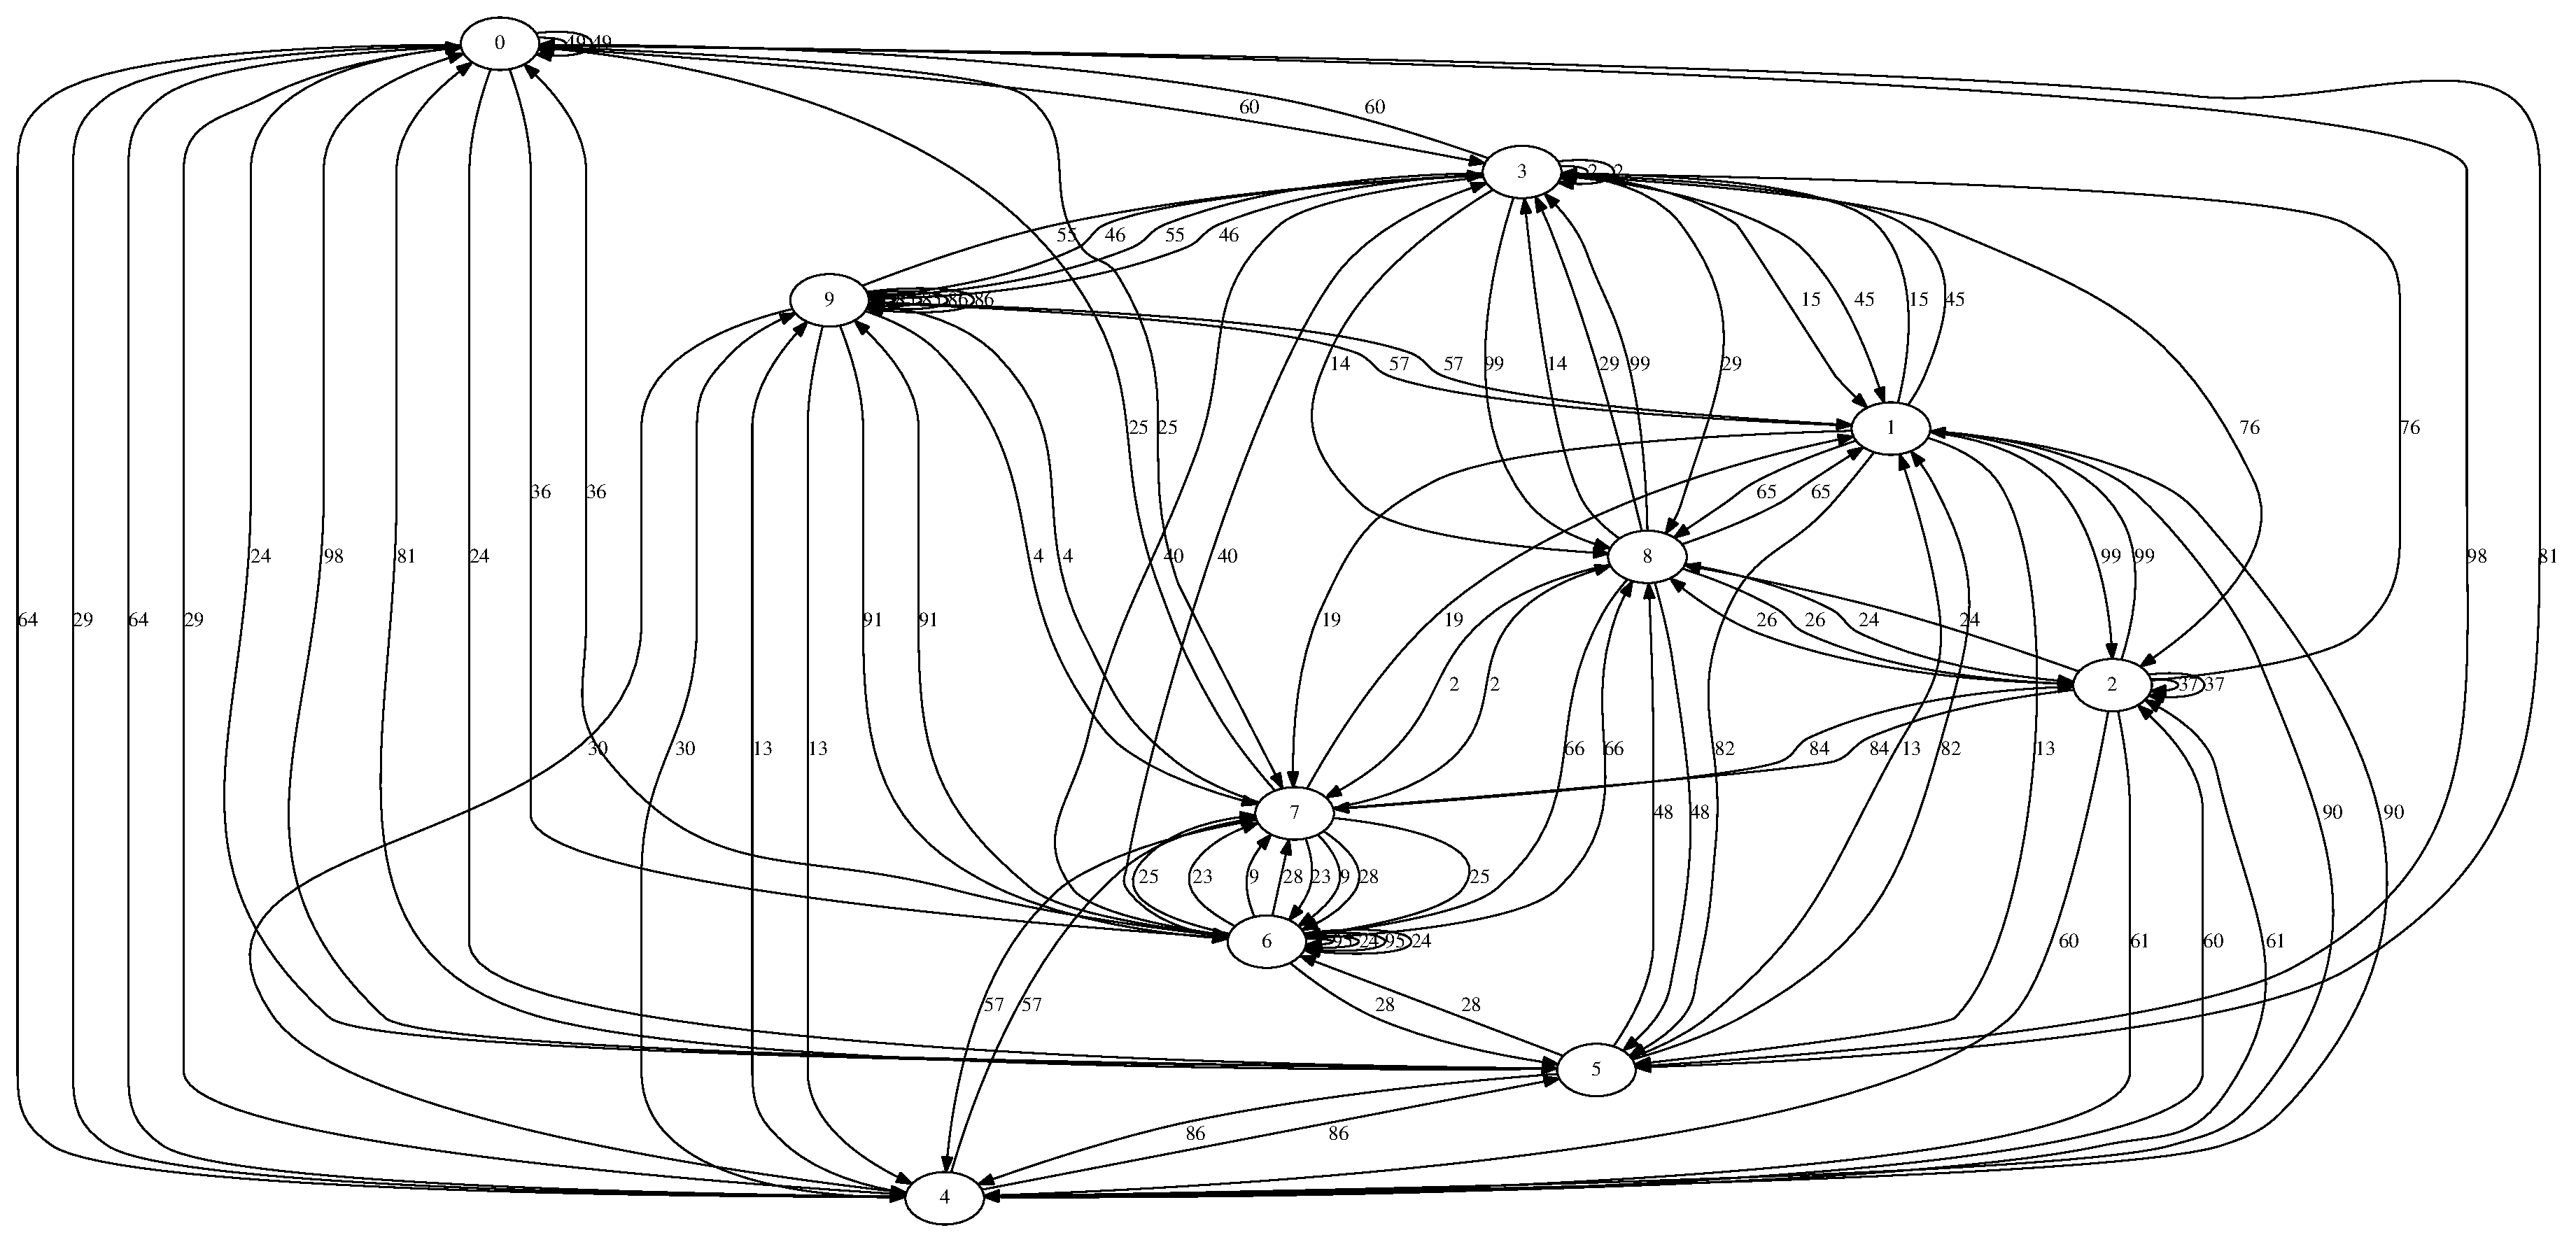
\includegraphics[width = 1\textwidth]{../prj/graf.dot.eps}
\caption{Przykładowy rysunek grafu dla 10 węzłów. Graf wykoanany za pomocą programu GrapViz, plik źródłowy: graf.dot}
\label{graf}
\end{figure} 


\end{document}
